\subsection{IP Checksum}

\begin{figure}
\begin{centering}
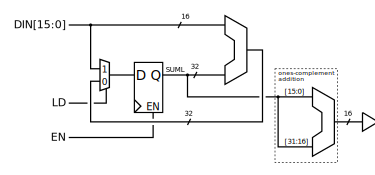
\includegraphics[scale=0.8]{ipchecksum.svg}
\end{centering}
\caption{IP Checksum Computation}
\label{ipchecksum}
\end{figure}

This module performs the IP Header checksum over a range of input words. 

The IP header checksum is defined by RFC 791 as

\begin{blockquote}
      The checksum field is the 16 bit one's complement of the one's
complement sum of all 16 bit words in the header.  For purposes of
computing the checksum, the value of the checksum field is zero.
\end{blockquote}

Ones-complement arithmetic can be implemented on twos-complement
hardware by adding the carry bit to the LSB.


\subsubsection{Interface}
To preload the checksum module with a value, place that value on
\signal{DIN[15:0]} and assert both \signal{LD} and \signal{EN}. To
update the checksum with the current value in \signal{DIN[15:0]}
assert \signal{EN}. Updates to \signal{CHKOUT[15:0]} are valid the
cycle after the assertion of \signal{EN}.

\subsection{UDP Header Writer}

For UDP event transmission, UDP data transmission, and event reception
response we need to craft UDP packets. The UDP header writer fills
this need by writing the appropriate input parameters to the correct
locations in an output ememory buffer. The buffer must be a full
frame, with frame length stored at location 0, and be sixteen bits
wide. All constant header fields (such as protocol number and TTL)
must be written to the buffer by other means -- it is assumed that
they will typically be hard-coded as initialization values and never
overwritten.


The header writer also computes the correct value for the length
fields as well as the IP header checksum.

\subsubsection{Interface}
The assertion of \signal{START} begins the header-writing process, which upon completion asserst \signal{DONE}. 

The input signals are

\begin{itemize}
\item \signal{DESTMAC[47:0]} : Destination MAC address
\item \signal{DESTIP[31:0]} : Destination IP address
\item \signal{SRCMAC[47:0]} : Source MAC address
\item \signal{SRCIP[31:0]} : Source IP address
\item \siganl{DESTPORT[15:0]} : Destination UDP port. 
\item \signal{WLEN[8:0]} : the 16-bit word length of the UDP datagram's body. 
\end{itemize}

\subsubsection{Implementation}

The ultimate implementation is a simple mux (Figure \ref{udpheaderwriter})  and FSM (Figure \ref{updheaderwriter.fsm}) which cycles through the correct input words and addresses and writes them to the buffer, finally writing the correctly-computed checksum. 


\begin{figure}
\begin{centering}
\includegraphics[scale=0.8]{udpheaderwriter.svg}
\end{centering}
\caption{UDP Header Writer.}
\label{udpheaderwriter}
\end{figure}

\begin{figure}
\begin{centering}
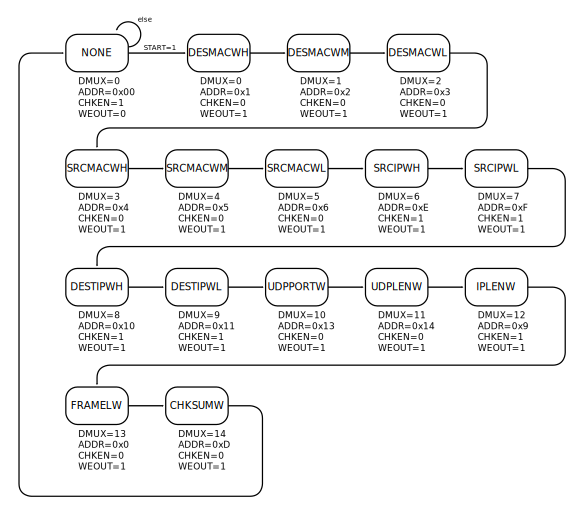
\includegraphics[scale=0.8]{udpheaderwriter.fsm.svg}
\end{centering}
\caption{UDP Header Writer FSM.}
\label{udpheaderwriter.fsm}
\end{figure}
